Subsection goes here.

In order to investigate the effect of argon plasma on waveguide quality,
waveguide loss measurement using the Fabry-Perot fringe technique were
performed. 3-$\mu$m-wide ridge waveguides were fabricated on the intermixed
region. The sample was then cleaved to form a 1-mm-long Fabry-Perot cavity.
A tunable (1.45-1.59$\mu$m) laser diode was used for the absorption experiments.
The light was modulated at 10KHz and coupled into the TE mode of the
waveguide through a tapered polarization preserving fiber. The transmitted
light was then captured by a similar fiber coupled to a Ge-detector followed
by a lock-in amplifier.

\begin{figure}[!t]
    \centering
    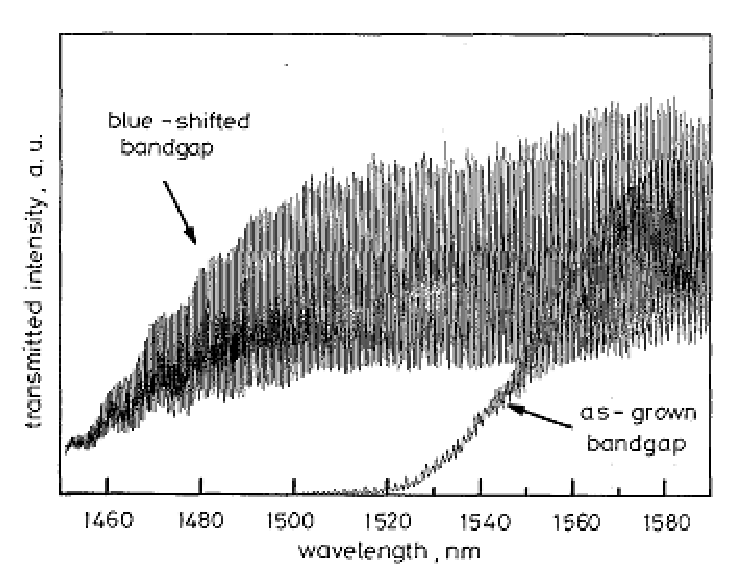
\includegraphics[width=2.5in]{fig/waveguide1}
    \caption{Measured transmission spectra of blue-shifted waveguide}
    \label{ex_waveguide1}
\end{figure}
Figure \ref{ex_waveguide1} shows the measured transmitted spectra of the blue-shift
waveguide cavity. Fabry-Perot interference fringes were formed due to multiple
reflections at the cleaved facets. From the contrast of these fringe the waveguide
loss can be determined by Equation \ref{loss},

\begin{equation}\label{loss}
    L=10\lg\Big[\frac{1}{\sqrt{R_1R_2}}\frac{1}{K_m}(1-\sqrt{1-K_m^2})\Big]
\end{equation}
where $R_1$ and $R_2$ are the reflectivity of the cleaved facets
and $K_m$ is the contrast of the fringes.

\begin{figure}[!t]
    \centering
    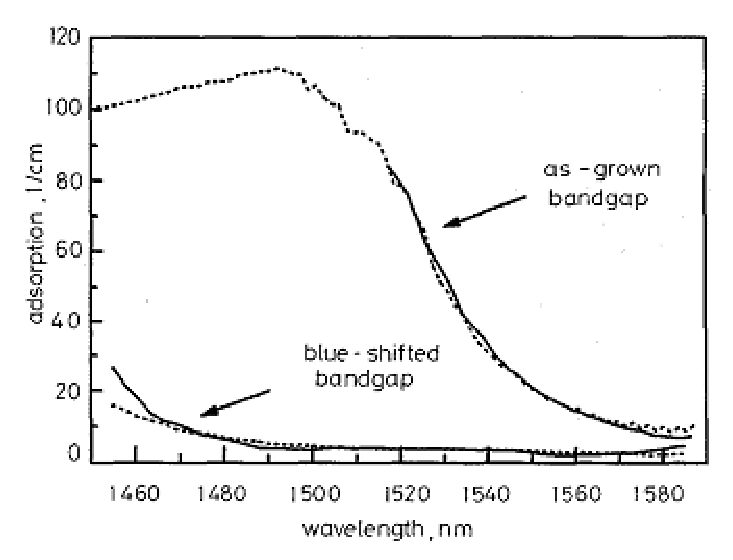
\includegraphics[width=2.5in]{fig/waveguide2}
    \caption{Absorption constants derived from measured transmission spectra
        using modulation ratio and average transmission intensity for
        blue-shifted waveguide}
    \label{ex_waveguide2}
\end{figure}
Figure \ref{ex_waveguide2} presents the absorption as a function of wavelength
derived from Figure \ref{ex_waveguide1} and Equation \ref{loss}.
